\documentclass{article}
\pagestyle{plain}
\setlength\textwidth{266.0pt}
\usepackage{amsmath}
\usepackage{amsthm}
\usepackage{amssymb}
\usepackage{mathrsfs}
\usepackage{graphicx}
\usepackage{epstopdf}
\usepackage{subfigure}
\usepackage{caption}
\usepackage{bm}
\usepackage{array}
\usepackage{multirow}
\usepackage[paperwidth=185mm,paperheight=260mm,text={148mm,220mm},left=21mm,top=25.5mm]{geometry}
\usepackage[round]{natbib}
\usepackage{booktabs}
\usepackage{algorithm,algpseudocode,amsmath}
\usepackage[colorlinks,linkcolor=blue,anchorcolor=blue,citecolor=blue]{hyperref}
\usepackage{color}
\usepackage{xcolor}
\usepackage{tikz}  
\usepackage{pdflscape}
 \newtheorem{thm}{Theorem}
\newtheorem{pro}{Proposition}
\newtheorem{lem}{Lemma}
\newtheorem{alg}{Algorithm}
\newtheorem{ass}{Assumption}
\newtheorem{coro}{Corollary}
\newtheorem{defin}{Definition}
\newtheorem{ob}{Observation}
\newtheorem{example}{Example}
\newtheorem{remark}{Remark}
%\newtheorem{proof}{Proof}
\usetikzlibrary{arrows,shapes,chains}  
\renewcommand{\algorithmicrequire}{\textbf{Input:}}  % Use Input in the format of Algorithm  
\renewcommand{\algorithmicensure}{\textbf{Output:}} % Use Output in the format of Algorithm  
\title {Review Notebook: Branch and Cut}
\author{CO2GENERATOR} 
\begin {document}
\maketitle 
\allowdisplaybreaks[4]

\section{Some Questions}

\noindent $\bullet$ How to use the Gomory's cutting plane method to solve the following integer programming problem?
\begin{align}
	\max \quad & 3x_1 - x_2 \\
	s.t. \quad & \left\{
	\begin{aligned}
		& 3x_1 - 2x_2 \leq 3 \\
		& 5x_1 + 4x_2 \geq 10 \\
		& 2x_1 + x_2 \leq 5 \\
		& x_1, x_2 \in \mathbb{Z}^+
	\end{aligned}\right.
\end{align}

\noindent $\bullet$ How to use the branch and bound method to solve the following integer programming problem?
\begin{align}
	\max \quad & 2x_1 + x_2 \\
	s.t. \quad & \left\{
	\begin{aligned}
		& x_1 + x_2 \leq 5 \\
		& -x_1 + x_2 \leq 0 \\
		& 6x_1 + 2x_2 \leq 21 \\
		& x_1, x_2 \in \mathbb{Z}^+
	\end{aligned}\right.
\end{align}

\noindent $\bullet$ What is branch-and-cut?

\newpage
\section{Cutting Plane}

Consider following integer programming problem,
\begin{align}
\label{problem:ip}
\begin{aligned}
\min \quad & c^Tx \\
s.t. \quad & Ax = b \\
& x \in \mathbb{Z}_+^n
\end{aligned}
\end{align}
And its linear relaxation is,
\begin{align}
\label{linear-relaxation}
\begin{aligned}
\min \quad & c^Tx \\
s.t. \quad & Ax = b \\
& x \in \mathbb{R}_+^n
\end{aligned}
\end{align}

Suppose the optimal solution obtained by (\ref{linear-relaxation}) is $x^*$ and given an optimal LP basis $B$, problem (\ref{problem:ip}) can be rewrote as,
\begin{align}
\min \quad & c_B^T B^{-1} b + \sum_{j \in NB} \bar{c}_jx_j \\
s.t. \quad & (x_B)_i + \sum_{j \in NB} \bar{a}_{ij}x_j = \bar{b}_i, && i = 1, 2, ..., m \\
& x_j \in \mathbb{Z}_+^1, && j = 1, 2, ..., n 
\end{align}
where $NB$ is the set of nonbasic variables. If $\forall i = 1, 2, ..., m$,  $\bar{b}_i$ is integer, then we obtain the optimal solution. Otherwise, there must be at least one $\bar{b}_i$ is fractional,
\begin{equation}
(x_B)_k + \sum_{j \in NB} \bar{a}_{kj}x_j = \bar{b}_k \label{fractional}
\end{equation}

 Since $x_j \geq 0$,
\begin{equation}
(x_B)_k + \sum_{j \in NB} \lfloor \bar{a}_{kj} \rfloor x_j \leq (x_B)_k + \sum_{j \in NB} \bar{a}_{kj}x_j  = \bar{b}_k
\end{equation}

Since $x_j$ should be integer,
\begin{equation}
(x_B)_k + \sum_{j \in NB} \lfloor \bar{a}_{kj} \rfloor x_j \leq \lfloor \bar{b}_k  \rfloor \label{vi}
\end{equation}

 Obviously, (\ref{vi}) is a valid inequality. Then, use (\ref{fractional}) and (\ref{vi}), we have
\begin{equation}
\sum_{j \in NB} (\bar{a}_{kj} - \lfloor \bar{a}_{kj} \rfloor) x_j \geq \bar{b}_k -  \lfloor \bar{b}_k  \rfloor \label{sub}
\end{equation}

Let $f_{kj} = \bar{a}_{kj} - \lfloor \bar{a}_{kj} \rfloor$, $g_k =  \bar{b}_k -  \lfloor \bar{b}_k\rfloor $, then we obtain the famous \textit{Chv\'atal-Gomory(C-G) Cut},
\begin{equation}
-\sum_{j \in NB} f_{kj} x_j \leq -g_k \label{cg-cut}
\end{equation}

 It is interesting. For the optimal solution $x^*$ of linear relaxation, the non-basic variables $x_j$ is zero and can't satisfy inequality (\ref{cg-cut}). Thus, such fractional solution will be cut off.
 
 \newpage
 \begin{example}
 	For the above integer programming problem (1)-(2), 
 	\begin{align*}
 	\max \quad & 3x_1 - x_2 \\
 	s.t. \quad & \left\{
 	\begin{aligned}
 	& 3x_1 - 2x_2 \leq 3 \\
 	& 5x_1 + 4x_2 \geq 10 \\
 	& 2x_1 + x_2 \leq 5 \\
 	& x_1, x_2 \in \mathbb{Z}^+
 	\end{aligned}\right.
 	\end{align*}
 	By introducing slack variables $x_3, x_4, x_5$, it can be converted to the following standard LP,
 	\begin{align*}
 		\max \quad & 3x_1 - x_2 \\
 		s.t. \quad & \left\{
 		\begin{aligned}
 		& 3x_1 - 2x_2 + x_3 = 3 \\
 		& 5x_1 + 4x_2 - x_4 = 10 \\
 		& 2x_1 + x_2 + x_5 = 5
 		\end{aligned}
 		\right.
 	\end{align*} 
 	Since both the left-hand-side(lhs) and $x_1, x_2, x_3$ are integral, the introduced slack variables must be integers. Then we can use the simplex algorithm to solve its linear programming relaxation. And the final optimal simplex tableau is,
 		\begin{table}[htbp]
	 		\centering
	 		\begin{tabular}{@{}ccccccccc@{}}
	 			\toprule
	 			\multicolumn{3}{c}{$c_j$}      & 3       & -1    & 0    & 0    & 0     & \multirow{2}{*}{$\theta$} \\ \cmidrule(r){1-8}
	 			$\bm{c_B}$     & $\bm{x}_B$     & $\bm{b}$       & $x_1$    & $x_2$ & $x_3$ & $x_4$ & $x_5$  &                        \\ \midrule
	 			3        & $x_1$     & 13/7      & 1       & 0    & 1/7    & 0    & 2/7     &                       \\
	 			-1        & $x_2$     & 9/7      & 0        & 1    & -2/7    & 0    & 3/7     &                       \\
	 			0        & $x_4$     & 31/7       & 0       & 0    & -3/7    & 1    & 22/7     &                       \\ \midrule
	 			\multicolumn{3}{c}{$c_j-z_j$} & 0       & 0    & -5/7    & 0    & -3/7     &                        \\  \bottomrule
	 		\end{tabular}%
 		\end{table}
 
  	Thus, we can introduce the following C-G cut,
	 \begin{equation}
	 -\frac{1}{7}x_3 - \frac{2}{7}x_5 \leq -\frac{6}{7}
	 \end{equation}
	 Then we introduce a new slack variable $x_6$ to continue the iteration.
	 \begin{equation}
	 -\frac{1}{7}x_3 - \frac{2}{7}x_5 + x_6 = -\frac{6}{7}
	 \end{equation}
	 And the simplex tableau is,
		\begin{table}[htbp]
		 	\centering
		 	\begin{tabular}{@{}cccccccccc@{}}
		 		\toprule
		 		\multicolumn{3}{c}{$c_j$}      & 3       & -1    & 0    & 0    & 0      &  0 & \multirow{2}{*}{$\theta$} \\ \cmidrule(r){1-9}
		 		$\bm{c_B}$     & $\bm{x}_B$     & $\bm{b}$       & $x_1$    & $x_2$ & $x_3$ & $x_4$ & $x_5$ & $x_6$ &                        \\ \midrule
		 		3        & $x_1$     & 13/7      & 1       & 0    & 1/7    & 0    & 2/7     &   0 &                    \\
		 		-1        & $x_2$     & 9/7      & 0        & 1    & -2/7    & 0    & 3/7     &     0 &                  \\
		 		0        & $x_4$     & 31/7       & 0       & 0    & -3/7    & 1    & 22/7     &     0 &                  \\ 
		 		0   & $x_6$      &  -6/7         &   0      &  0    & -1/7    & 0    & -2/7     &   1  &  \\ \midrule
		 		\multicolumn{3}{c}{$c_j-z_j$} & 0       & 0    & -5/7    & 0    & -3/7   &  0 &                    \\  \bottomrule
		 	\end{tabular}%
	 	\end{table}
 	
 	 Since $x_6 = -\frac{6}{7} \leq 0$ is not a feasible solution, but the dual problem is feasible. Therefore, here we should use dual-simplex method. After several iterations, the optimal simplex tableau is
 	 \begin{table}[htbp]
 	 	\centering
 	 	\begin{tabular}{@{}cccccccccc@{}}
 	 		\toprule
 	 		\multicolumn{3}{c}{$c_j$}      & 3       & -1    & 0    & 0    & 0      &  0 & \multirow{2}{*}{$\theta$} \\ \cmidrule(r){1-9}
 	 		$\bm{c_B}$     & $\bm{x}_B$     & $\bm{b}$       & $x_1$    & $x_2$ & $x_3$ & $x_4$ & $x_5$ & $x_6$ &                        \\ \midrule
 	 		3        & $x_1$     & 1      & 1       & 0    & 0   & 0    & 0     &   1 &                    \\
 	 		-1        & $x_2$     & 5/4      & 0        & 1    & 0    & -1/4    & 0     &  -5/4  &                  \\
 	 		0        & $x_3$     & 5/2       & 0       & 0    & 1    & -1/2    & 0     &  -11/2 &                  \\ 
 	 		0   & $x_5$      &  7/4         &   0      &  0    & 0    & 1/4    & 1     &   -3/4  &  \\ \midrule
 	 		\multicolumn{3}{c}{$c_j-z_j$} & 0       & 0    & 0    & -1/4    & 0   &  -17/4 &                    \\  \bottomrule
 	 	\end{tabular}%
 	 \end{table}
  
  	\
  	
  	\
  	
  	We can derive the C-G cut as,
  	\begin{equation}
  		-(\frac{1}{4} - 0)x_4 - (-\frac{3}{4} - -1)x_6 \leq -(\frac{7}{4} - 1)
  	\end{equation}
  	And introduce the slack variable $x_7$,
  	\begin{equation}
  		-\frac{1}{4} x_4 - \frac{1}{4}x_6 + x_7 = -\frac{3}{4}
  	\end{equation}
   Then, continue the iteration. Finally, we obtain the optimal simplex tableau,
   	\begin{table}[htbp]
	   	\centering
	   	\begin{tabular}{@{}ccccccccccc@{}}
	   		\toprule
	   		\multicolumn{3}{c}{$c_j$}      & 3       & -1    & 0    & 0    & 0      &  0     &  0   & \multirow{2}{*}{$\theta$} \\ \cmidrule(r){1-10}
	   		$\bm{c_B}$     & $\bm{x}_B$     & $\bm{b}$       & $x_1$    & $x_2$ & $x_3$ & $x_4$ & $x_5$ & $x_6$ &     $x_7$  &           \\ \midrule
	   		3        & $x_1$     & 1      & 1         & 0      & 0    & 0        & 0     &   1       &      0      &        \\
	   		-1        & $x_2$     & 2      & 0        & 1      & 0    & 0    & 0     &  -1  &    -1     &         \\
	   		0        & $x_3$     & 4       & 0       & 0      & 1    & 0    & 0     &  -5   &    -2    &          \\ 
	   		0       & $x_5$      &  1         &   0   &  0    & 0     & 0    & 1     &   -1   &    1    &    \\
	   		0       &  $x_4$      &  3       &   0    & 0     &  0    &    1      &   0    &  1     &   -4    &    \\ \midrule
	   		\multicolumn{3}{c}{$c_j-z_j$} & 0       & 0    & 0    & 0    & 0   &  -4   &     -1    &        \\  \bottomrule
	   	\end{tabular}%
   \end{table}

	And the optimal solution is $\bm{x} = (1, 2, 4, 3, 1, 0, 0)^T$.
\end{example}


\begin{remark}
	We have noticed that, when a new valid inequality is introduced, it is no need to restart the simplex process. The dual-simplex method can be employed to continue the optimization. It is critical important for improving computation efficiency, since it allows for warm start rather than cold start. And the same technique is also used in the branch and bound algorithm. And it is worth mention that, CPLEX/GUROBI use the dual-simplex method to solve the LP relaxation at every nodes of the search tree.
\end{remark}


\newpage
\section{Branch and Bound}

Take the following problem as an example,
\begin{align}
\min \quad & 4x_1 + 9x_2 + 6x_3 \\
s.t. \quad & 5x_1 + 8x_2 + 6x_3 \geq 12 \\
& x_1, x_2, x_3 \in \left\{0, 1\right\}
\end{align}
The optimal solution is $(1, 1, 0)$, objective is $13$. And its linear relaxation,
\begin{align}
\min \quad  4x_1 + 9x_2 + 6x_3 \qquad\qquad  \\
s.t. \quad \left\{
\begin{aligned}
& \quad 5x_1 + 8x_2 + 6x_3 \geq 12 \\
& \quad 0 \leq x_1 \leq 1 \\
& \quad 0 \leq x_2 \leq 1 \\
& \quad 0 \leq x_3 \leq 1 \\
& \quad x_1, x_2, x_3 \in \mathbb{R}
\end{aligned} \right.
\end{align}
The optimal solution is $(1, 0.125, 1)$, objective is $11.125$. Thus, \textit{Branch and Bound} can be illustrated as,

\begin{figure}[htbp]
	\centering
	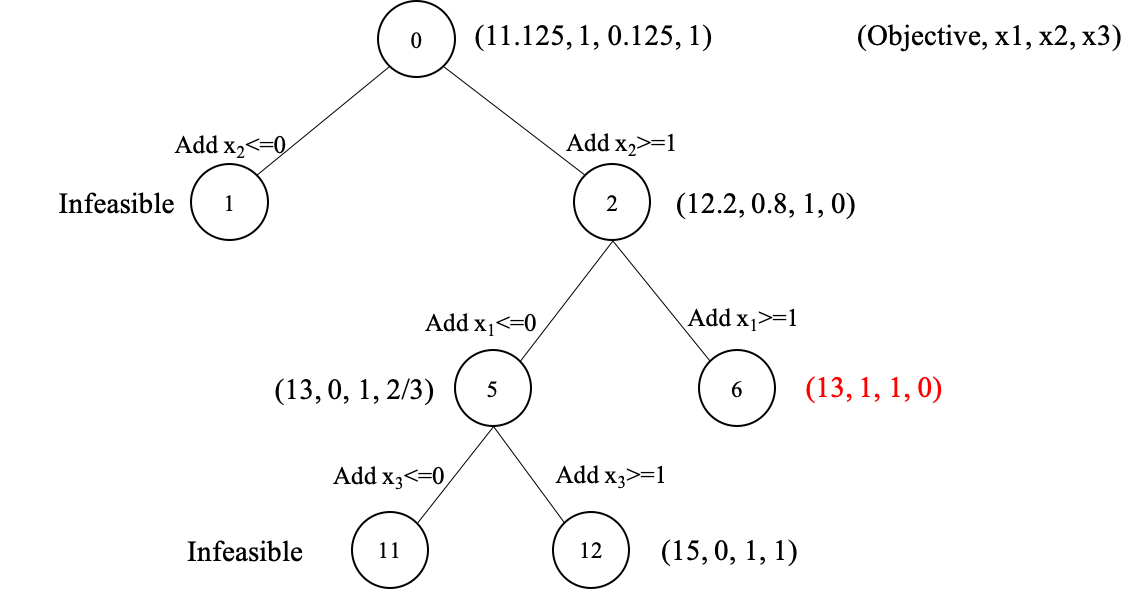
\includegraphics[width=0.8\linewidth]{./figure/rn-b-a-c-tree.png}
	\caption{Search Tree of Above Problem}
	\label{fig:bb}
\end{figure}

\noindent The generic branch and bound algorithm can be described as,
\begin{algorithm}[htbp]
	\caption{Generic Branch and Bound Algorithm}
	\label{alg:bb}
	\begin{algorithmic}[1]
		\State Set $U = +\infty$ and break the original problem into two subproblems
		\State Select an active subproblem
		\State If the subproblem is infeasible, delete it; otherwise, compute $b(F)$ for the corresponding subproblem as a lower bound.
		\State If $b(F) \geq U$, delete the subproblem
		\State If $b(F) < U$, either obtain an optimal solution to subproblem, or break the corresponding subproblem into further subproblems, which are added to the list of active subproblems
		\State Repeat 2$\sim$5, until there is no active subproblem.
	\end{algorithmic}  
\end{algorithm} 

\newpage
\section{Branch and Cut}

\begin{figure}[htbp]
	\centering
	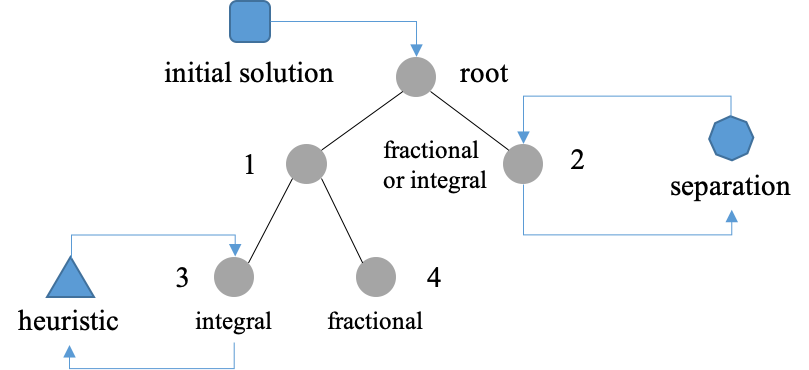
\includegraphics[width=0.7\linewidth]{figure/rn-b-a-c-framework}
	\caption{An illustration for the branch-and-cut framework.}
	\label{fig:rn-b-a-c-framework}
\end{figure}


\section{Conclusion}


% \newpage
% \bibliographystyle{chicago}
% \bibliography{reference}
\end {document} 